%%%%%%%%%%%%%%%%%%%%%%%%%%%%%%%%%%%%%%%%%%%%%%%%%%%%%%%%%%%%%%%%%%%%%%%%%%%%%%%%%%%%%%%%%%%%%%%%%%%%%
% baposter Landscape Poster
% LaTeX Template
% Version 1.0 (11/06/13)
%
% baposter Class Created by:
% Brian Amberg (baposter@brian-amberg.de)
%
% This template has been downloaded from:
% http://www.LaTeXTemplates.com
%
% License:
% CC BY-NC-SA 3.0 (http://creativecommons.org/licenses/by-nc-sa/3.0/)
%
%%%%%%%%%%%%%%%%%%%%%%%%%%%%%%%%%%%%%%%%%%%%%%%%%%%%%%%%%%%%%%%%%%%%%%%%%%%%%%%%%%%%%%%%%%%%%%%%%%%%%

%----------------------------------------------------------------------------------------------------
%	PACKAGES AND OTHER DOCUMENT CONFIGURATIONS
%----------------------------------------------------------------------------------------------------

\documentclass[landscape,a0paper,fontscale=0.32]{baposter} % Adjust the font scale/size here

\usepackage{listings}
\usepackage{tabu}

\usepackage{wrapfig}
\usepackage{graphicx} % Required for including images
\graphicspath{{figures/}} % Directory in which figures are stored

\usepackage{amsmath} % For typesetting math
\usepackage{amssymb} % Adds new symbols to be used in math mode

\usepackage{booktabs} % Top and bottom rules for tables
\usepackage{enumitem} % Used to reduce itemize/enumerate spacing
\usepackage{palatino} % Use the Palatino font
\usepackage[font=small,labelfont=bf]{caption} % Required for setting captions to tables and figures

\usepackage{multicol} % Required for multiple columns
\setlength{\columnsep}{1.5em} % Slightly increase the space between columns
\setlength{\columnseprule}{0mm} % No horizontal rule between columns

\usepackage{tikz} % Required for flow chart
\usetikzlibrary{shapes,arrows} % Tikz libraries required for the flow chart in the template

% Define a command to reduce spacing within itemize/enumerate environments,
% this is used right after \begin{itemize} or \begin{enumerate}
\newcommand{\compresslist}{
\setlength{\itemsep}{1pt}
\setlength{\parskip}{0pt}
\setlength{\parsep}{0pt}
}

\definecolor{lightblue}{rgb}{1,0,0} % Defines the color used for content box headers

\begin{document}

\begin{poster}
{
headerborder=closed, % Adds a border around the header of content boxes
colspacing=1em, % Column spacing
bgColorOne=white, % Background color for the gradient on the left side of the poster
bgColorTwo=white, % Background color for the gradient on the right side of the poster
borderColor=lightblue, % Border color
headerColorOne=black, % Background color for the header in the content boxes (left side)
headerColorTwo=lightblue, % Background color for the header in the content boxes (right side)
headerFontColor=white, % Text color for the header text in the content boxes
boxColorOne=white, % Background color of the content boxes
% Format of the border around content boxes,
% can be: none, bars, coils, triangles, rectangle, rounded, roundedsmall, roundedright or faded
textborder=rounded,
eyecatcher=true, % Set to false for ignoring the left logo in the title and move the title left
headerheight=0.1\textheight, % Height of the header
% Specify the rounded corner in the content box headers,
% can be: rectangle, small-rounded, roundedright, roundedleft or rounded
headershape=roundedright,
headerfont=\Large\bf\textsc, % Large, bold and sans serif font in the headers of content boxes
%textfont={\setlength{\parindent}{1.5em}}, % Uncomment for paragraph indentation
linewidth=2pt, % Width of the border lines around content boxes
columns=4
}
%----------------------------------------------------------------------------------------------------
%	TITLE SECTION
%----------------------------------------------------------------------------------------------------
{
\includegraphics[height=4em]{left_logo}} % First university/lab logo on the left
{\bf\textsc{Fast and Correct}\vspace{0.5em}} % Poster title
{\textsc{ {\Large \{Mark Baranowski, Ian Briggs, Ganesh Gopalakrishnan, Zvonimir Rakamaric\}}\\
    \hspace{12pt} University of Utah School of Computing}} % Authors and institution
{
\includegraphics[height=4em]{right_logo}} % Second university/lab logo on the right











%----------------------------------------------------------------------------------------------------
% Introduction/Motivation
%----------------------------------------------------------------------------------------------------
\headerbox{Motivation}{name=BoxOne,column=0,span=1}{
  % Intro/Motivation can be the importance of glob opt in many contexts including
  % FP error bounding and FP error bounding can be motivated via its relevance to
  % HPC code precision tuning

  %% Floating point computation is inherently flawed. Each operation carries with it an error term
  %% that, with many operations compounding, can cause tremendous error in the output. When using
  %% floating point arithmetic one must be aware of the magnitude of the error in the computation being
  %% done. This is where floating point error bounding comes into play. It can be used to give tight
  %% upper bounds to computations, such as those used in high powered computing. To power this bounding
  %% is global optimization utilizing interval arithmetic.

  Floating point computation is, at its core, an approximation. Errors due to this approximation can
  cause programs to malfunction when not accounted for.
  \begin{itemize}\compresslist
  \item The Large Hadron Collider had error occur when switching math libraries which caused many
    missed and miss-identified collisons. \cite{bailey2013high}
  \item The targeting program for the Patriot missle accumulated a floating point error which
    caused the death of 28 American soldiers \cite{blair1992patriot}, which accounts for $19\%$
    of U.S. casualties in the war \cite{leland2010american}.
  \end{itemize}
  FPTaylor \cite{fm2015-sjrg} is a tool which can determine the maximum error of a floating point
  function. Unlike other tools in this domain it can handle transcendental opetators. The downside
  of this tool, up to this point, is speed. The global maxima solver in the tools core can be sped up
  through parallelization.
  % When there are two boxes, some whitespace may need to be added if the
  % one on the right has more content
  % \vspace{0.3em}
}





%----------------------------------------------------------------------------------------------------
% Serial Algorithm
%----------------------------------------------------------------------------------------------------
\headerbox{Serial Algorithm}{name=BoxTwo, column=0, span=1, below=BoxOne}{
  %% The classical branch and bound algorithm utilizes the property of interval arithmetic that
  %% computation of a function over an interval gives an answer bound that is guaranteed to contain the
  %% real bounds of the function within the inputs given. A high water mark is used to store the highest
  %% lower bound seen, and if a given input produces an output which lies completely below this mark
  %% then the input can be discarded. Otherwise the input is split in half and this computation is
  %% repeated on each new input. An input will also be discarded if the maximum width is below a user
  %% set threshold. Once there are no more inputs to process the maximum of the function is tightly
  %% bounded by the highest upper output of the inputs which were discarded due to width tolerance.
  The function generated by FPTaylor characterizes the error of the input computation. To find the
  maxima of this function within a seach space a brach and bound algorithm is used. It utilizes the
  inclusion property of interval arithmatic.
  \small{
  \begin{lstlisting}[language=Python]^^J
while\ queue.not\_empty:\ ^^J
\ \ x\ =\ queue.get^^J
\ \ y\ =\ f(x)^^J
\ \ if\ (y.width\ <\ threshold)\ and^^J
\ \ \ \ \ (y.upper\ >\ answer):^^J
\ \ \ \ answer\ =\ output.upper\ ^^J
\ \ if\ y.upper\ <\ high\_water\_mark:^^J
\ \ \ \ continue\ ^^J
\ \ for\ xi\ in\ search\_space.bisect:^^J
\ \ \ \ yi\ =\ f(xi.midpoint)^^J
\ \ \ \ if\ yi.lower\ >\ high\_water\_mark:^^J
\ \ \ \ \ \ high\_water\_mark\ =\ yi.lower^^J
\ \ \ \ queue.put(xi)^^J
  \end{lstlisting}
  }

  % When there are two boxes, some whitespace may need to be added if the
  % one on the right has more content
  % \vspace{0.3em}
}





%----------------------------------------------------------------------------------------------------
% Swig
%----------------------------------------------------------------------------------------------------
\headerbox{Swig}{name=BoxThree, column=0, below=BoxTwo, above=bottom}{
  To utilize existing libraries for performing interval arithmetic we used the MPFI library. To
  allow for quick prototyping we elected to use Python as the language for the main algorithm. In
  order to interface these two language we used the Simplified Wrapper and Interface Generator, SWIG.
  This quick prototyping allowed leeway for ideas to be quickly tested before much work went into
  them. Python was never meant to be the end target, just a way to query the field of ideas quickly
  so a suitable algorithm could be found for the final product.
  % When there are two boxes, some whitespace may need to be added if the
  % one on the right has more content
  % \vspace{0.3em}
}



















%----------------------------------------------------------------------------------------------------
% Example Parallel Algorithms
%----------------------------------------------------------------------------------------------------
\headerbox{Example Parallel Algorithms}{name=BoxFour, column=1, span=2}{
  %% There is considerable shared state in the traditional algorithm. The high water mark, the inputs
  %% which are still to be processed, and the maximum as it is found. To mitigate the problems
  %% associated with shared state we experimented with various methods. One consisted of using parallel
  %% map functions on a list of the inputs to be process, each map produced a list of new inputs, a list
  %% of new high water marks, and a list of new solutions. The latter two were reduced to find the
  %% maximum and the process repeated. Another solver split the initial input into many pieces and sent
  %% those off to worker threads. When a worker thread finished work on it's input it would report back
  %% to the main thread with a new water mark and maximum, if found, and the main thread would in turn
  %% given the thread a new input to work on. If the new values were better than the main threads values
  %% an update would be issued to all worker threads to update their local values. 
  \begin{tabu}{p{.316\linewidth}p{.316\linewidth}p{.316\linewidth}}
    \rowfont[l]{\large\bfseries} Map & Input Splitting & Input Oversplitting \\
    \rowfont[l]{}
    \begin{itemize}[leftmargin=10pt, topsep=0pt]\compresslist
    \item Utilize a parallel map over a list of current search spaces.
    \item The function return is a triple of new sarch spaces, new high water mark, and new answer.
    \item The new search spaces are put into the next list of search spaces.
    \item The high water mark and answers are updated to be the max of their respective returned values.
    \end{itemize}
    &
    \begin{itemize}[leftmargin=10pt, topsep=0pt]\compresslist
    \item Split it initial search area into $t$ pieces.
    \item Run the serial algorithm for each sub-problem.
    \item When all return take the maximum of the returns as the answer.
    \end{itemize}
    &
    \begin{itemize}[leftmargin=10pt, topsep=0pt]\compresslist
    \item Split the initial search space into many pieces.
    \item Start $t$ serial solvers modified to return the high water mark as well.
    \item When a solver returns give it a new piece.
    \item If the returned high water mark is better than the current then issue an update to all other workers.
    \end{itemize}
  \end{tabu}
  % When there are two boxes, some whitespace may need to be added if the
  % one on the right has more content
  % \vspace{0.3em}
}





%----------------------------------------------------------------------------------------------------
% Runtime comparison of solvers
%----------------------------------------------------------------------------------------------------
\headerbox{Runtime}{name=BoxFive, column=1, span=2, below=BoxFour}{
  \begin{centering}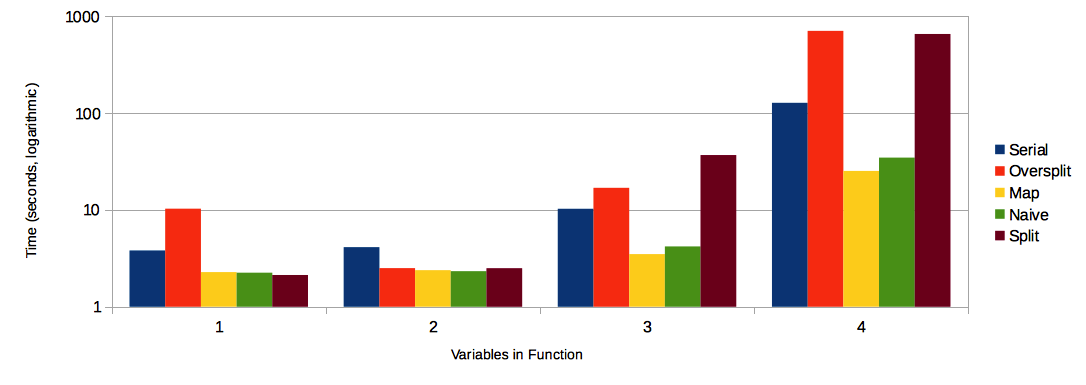
\includegraphics[width=\linewidth]{graph_one}\end{centering}
  % When there are two boxes, some whitespace may need to be added if the
  % one on the right has more content
  % \vspace{0.3em}
}





\newlength{\graphWidth}
\setlength{\graphWidth}{2in}
%----------------------------------------------------------------------------------------------------
% Function complexity vs time graph
%----------------------------------------------------------------------------------------------------
\headerbox{Function Complexity}{name=BoxSix, column=1, span=2, below=BoxFive, above=bottom}{
  \begin{tabular}{p{\graphWidth}p{.95\linewidth-2\graphWidth}p{\graphWidth}}
    \raisebox{-.9\totalheight}{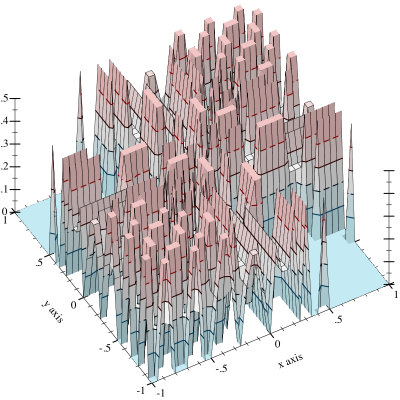
\includegraphics[width=\graphWidth]{graph_two}}
    \captionof{figure}{Error for $a+b$}
    &
    \begin{enumerate}[topsep=0pt]\compresslist
    \item Error in floating point operations is highly erratic
    \item This makes them ill-conditioned for optimization
    \item Search space is exponential in the number of input dimentions
    \item Utilizing seperable partitions of the function can be usable
      \begin{enumerate}\compresslist
      \item Creating less complex subproblems
      \item This can only be used for seperable functions
      \end{enumerate}
    \end{enumerate}
    %% The number of input variables to a function causes an exponential increase in the search space
    %% and solving time. There are tricks to tame this complexity. Partitioning the function into
    %% expressions which contain no overlapping variables is one example. The problem with these
    %% simplifications is that they only apply to a subset of input functions. If the function cannot
    %% be split into expressions it must be solved as a whole.
    &
    \raisebox{-.9\totalheight}{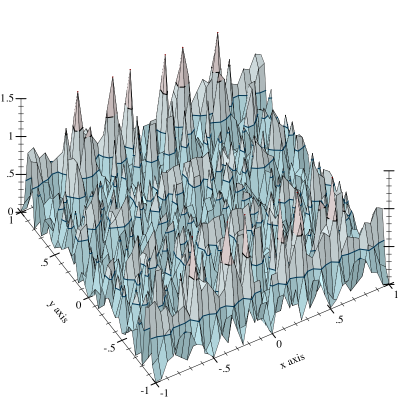
\includegraphics[width=\graphWidth]{graph_three}}
    \captionof{figure}{Error for $a*sin(b)$}
  \end{tabular}
  % When there are two boxes, some whitespace may need to be added if the
  % one on the right has more content
  % \vspace{0.3em}
}


























%----------------------------------------------------------------------------------------------------
% Python Complications
%----------------------------------------------------------------------------------------------------
\headerbox{Python Complications}{name=BoxSeven, column=3}{
  %% The multiprocessing module for python has inconsistent costs for operations when compared to other
  %% languages.A shared Ctype variable is very fast while a shared variable of any other type is quite
  %% costly. For the latter to manage shared memory a process is used to pass information between the
  %% worker process. This is hidden from the programmer. Shared queues are far faster unless certain
  %% operators are used in sequence, such as placing multiple items in a queue then accessing the member
  %% variable not\_empty. While the flexibility to experiment with ideas was useful, there are some
  %% drawbacks.
  Python has no proper multithreading ability, instead processes are used. To compound on this there
  are inconsistent costs for operations.
  \begin{itemize}\compresslist
  \item \emph{Ctype}, an unchangable list of build in types, varaibles are quite fast to share while
    most other types are orders of magnatude slower
  \item Share namespaces are handled via communication with a sentinal process
  \item Shared queues are faster than a shared namespace with one object in it
  \item But, a queue can slow down incredibly if accessing the \lstinline{not_empty} member
    variable
  \end{itemize}

  There are also precautions that need to be taken when using SWIG with python.
  \begin{itemize}\compresslist
  \item All libraries used in the C++ code being wrapped must be compiled as shared libraries
  \item Violation of memory safety is not always apparent in the python code
  \item Types cannot cross SWIG interface boundaries, i.e. If the same C++ class is wrapped by two
    different SWIG interfaces they are not interoperable in python
  \end{itemize}
  % When there are two boxes, some whitespace may need to be added if the
  % one on the right has more content
  % \vspace{0.3em}
}





%----------------------------------------------------------------------------------------------------
% Move to Rust
%----------------------------------------------------------------------------------------------------
\headerbox{Move to Rust}{name=BoxEight, column=3, below=BoxSeven}{
  To aid in the overall speed of our optimization we are turning to Rust. This allows us to still
  leverage C and C++ interval libraries while having a more hospitable enviroment, due to the
  similarities between Rust and C. From our testing this has shown to be very promising giving us:
  \begin{itemize}\compresslist
  \item Faster compilation
  \item Less time for small allocations, the bulk of our memory use
  \item Inherent memory safety
  \item Low level control for setting rounding modes
  \end{itemize}
  % When there are two boxes, some whitespace may need to be added if the
  % one on the right has more content
  % \vspace{0.3em}
}



%----------------------------------------------------------------------------------------------------
% References
%----------------------------------------------------------------------------------------------------

\headerbox{References}{name=BoxNine, column=3, below=BoxEight, above=bottom}{
\renewcommand{\section}[2]{\vskip 0.05em} % Get rid of the default "References" section title
\nocite{*} % Insert publications even if they are not cited in the poster
\scriptsize{ % Reduce the font size in this block
\bibliographystyle{unsrt}
\bibliography{biblio} % Use sample.bib as the bibliography file
}
  % When there are two boxes, some whitespace may need to be added if the
  % one on the right has more content
  % \vspace{0.3em}
}






\end{poster}

\end{document}
